\chapter{Nanorods}

\label{ch:nanorod}

\section{Purpose}

As noted in Chapter~\ref{ch:selective}, the team faced significant difficulties creating a nonlinear signal for use in NLTR.  The team investigated the use of ferromagnetic nanorods to generate a nonlinear signal.

\section{Methodology}
\label{sec:nanorod-meth}

An additional experiment was conducted by the team to determine whether ferromagnetic nanorods could generate a useable nonlinear signal for nonlinear time reversal. For the first experiment, the ferromagnetic nanorods were attached with tape to a monopole antenna and put into a small box lined with tin foil that acts as a reflective chamber. This was attached via a circulator in sequence with a signal generator and a spectrum analyzer (as shown in Figure~\ref{fig:nanorod-setup}). The signal generator output a CW, which swept from \numrange{1}{10}~GHz every .5~GHz.

\begin{figure}[h!]
\centering
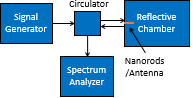
\includegraphics[width=0.85\textwidth]{nanorod/setup}
    \caption[Initial ferromagnetic nanorod experimental setup]{Diagram showing connections between the antenna, signal generator, and spectrum analyzer used in the first experimental setup.}
    \label{fig:nanorod-setup}
\end{figure}

The next step in this research was to move to Gigabox testing. The setup for this experiment followed that of the first step of linear time reversal, with modifications to the responding antenna depending on the iteration of the variable being tested.

In the first round of testing, a simple pole antenna was used, with the ferromagnetic nanorods being taped to the transmitting antenna. The DSO then collected the signal from the transmitting antenna at a port several centimeters away.

After initial tests with the control variable being the presence of the ferromagnetic nanorods, the next test compared the base behavior of the antenna to the response of the ferromagnetic nanorods in the presence of a magnetic field. In order to accomplish this, a magnet was affixed to the outside of the Gigabox as close to the transmitting port as possible. In each of these first two tests, the frequency was swept every .1~GHz from 3.5~GHz to 6.5~GHz.

\begin{figure}[h!]
\centering
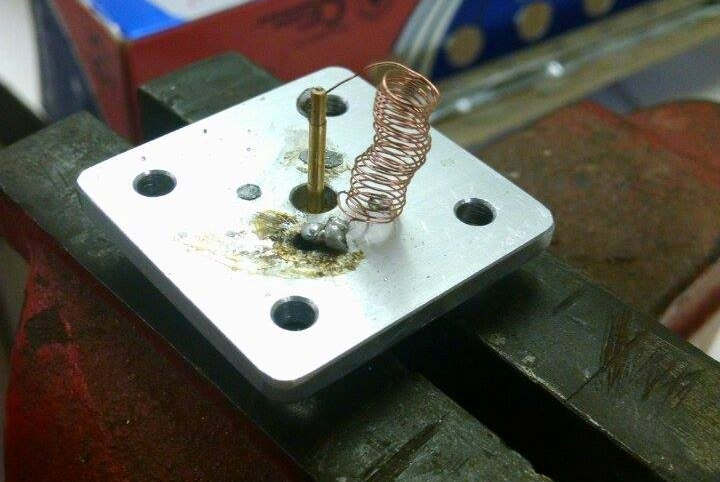
\includegraphics[width=0.85\textwidth]{nanorod/antenna}
    \caption[Antenna used with ferromagnetic nanorods in the Gigabox]{The ferromagnetic nanorods are affixed inside the copper solenoid, which is placed beside the antenna in order to test a different alignment of the magnetic field.}
    \label{fig:nanorod-setup}
\end{figure}

The third and final test relied on the same magnetic stimulation as the second iteration of the Gigabox test, with a different antenna, this one fashioned into a solenoid, to test a different alignment of the magnetic field. This final round of testing had the highest frequency resolution, which swept from 3.05 GHz to 6 GHz at every .05 GHz. For additional certainty, the measurements from five runs were averaged for a final result.

In each of the above tests, the carrier frequency was the independent variable swept across. This is represented as 1F. The dependent variable was the recorded voltage at the nonlinear frequency, 2F, double the carrier frequency. This voltage was separated using an FFT function in Matlab.

\section{Results}
\label{sec:nanorod-results}

\begin{figure}[h!]
    \centering
    \begin{subfigure}{0.45\textwidth}
        \centering
        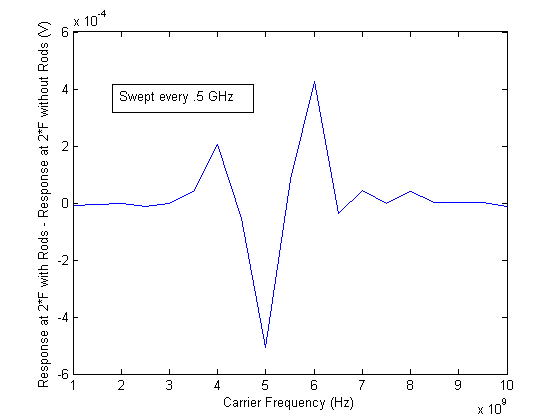
\includegraphics[width=1.0\linewidth]{nanorod/exp-1}
        \caption[]{}
        \label{nanorod-exp-1}
    \end{subfigure}
        \begin{subfigure}{0.45\textwidth}
        \centering
        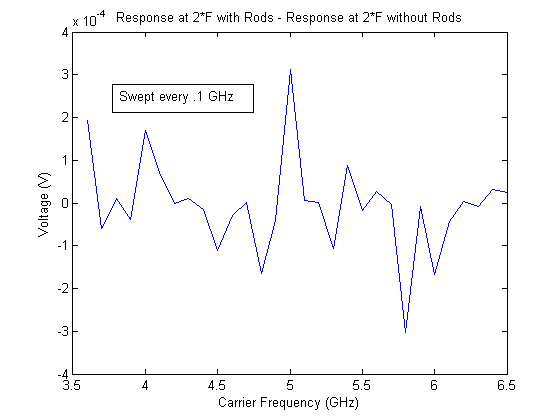
\includegraphics[width=1.0\linewidth]{nanorod/exp-2}
        \caption[]{}
        \label{nanorod-exp-2}
    \end{subfigure}
        \begin{subfigure}{0.45\textwidth}
        \centering
        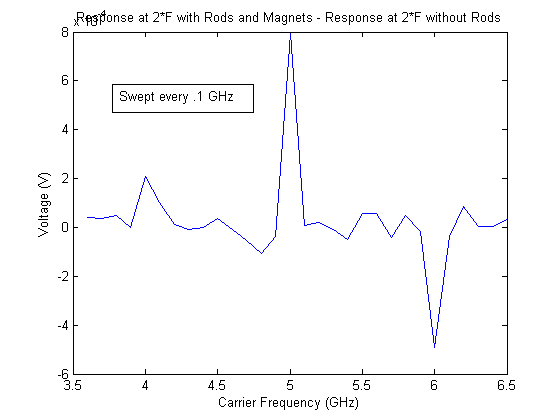
\includegraphics[width=1.0\linewidth]{nanorod/exp-3}
        \caption[]{}
        \label{nanorod-exp-3}
    \end{subfigure}
        \begin{subfigure}{0.45\textwidth}
        \centering
        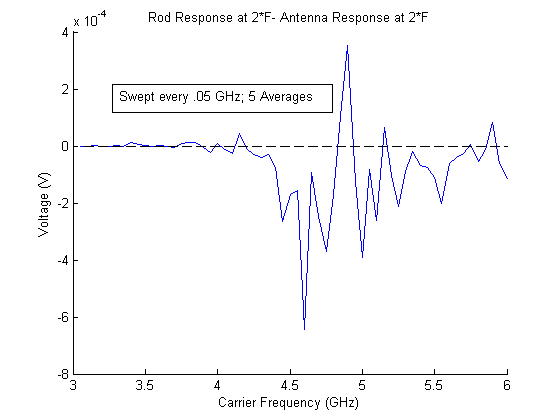
\includegraphics[width=1.0\linewidth]{nanorod/exp-4}
        \caption[]{}
        \label{nanorod-exp-4}
    \end{subfigure}
    \caption[Ferromagnetic nanorod experimental results]{Experimental results}
    \label{fig:nanorod-results}
\end{figure}

Figure~\ref{fig:nanorod-exp-1} shows positive spikes in nanorod response compared to the base at 4 GHz and 6 GHz. Contrast this to Figures 8 and 9 below; they show a sharp peak in nonlinear response with the ferromagnetic nanorods at 5 GHz, where the sharp dip in performance occurred in the first test.

Figure~\ref{fig:nanorod-exp-4} shows the final results with the loop antenna and magnetic stimulation, with behavior averaged across five tests. This is also the finest resolution, taken in the areas of interest from the results of the previous tests.

\section{Discussion}
\label{sec:nanorod-discussion}

\todo{Instead of saying we found some results, say we can conclude from the figures that it's all noise and that we can't conclude anything and just leave it at that and then talk about future work. It's okay to say we couldn't get a signal, much better than BSing.}

The results show a general attenuation response in the gigahertz range of transmission for the ferrite ferromagnetic nanorods. The first test involving the small foil-lined box showed an extremely attenuated response at all frequencies. The level of attenuation seems to indicate that the ferromagnetic nanorods have no significant nonlinear response. Higher frequencies might provide a more significant response, though this would require different equipment than what is currently available.

\todo{Remember to resolve the ?? #'s for the figures in 10.3 and elsewhere!}
